\chapter{Strategies for splitting a matrix $A$ into $A_r$ and $A_c$} \label{chap:methods}

The main goal of this thesis is to find efficient ways of splitting our original matrix $A$ into $A_r$ and $A_c$, in order to use the medium-grain model.

We are interested in both improving the initial partitioning of $A$, and a fully iterative method; therefore, we will make the distinction between methods that don't need an initial partitioning (\emph{partition-oblivious} methods), and are therefore suitable for the first case, and methods that do require an initial partitioning (\emph{partition-aware} methods), to be used in a fully iterative scheme. Most of the time the same algorithm can be used for both purposes, albeit with slight modifications.  Before we proceed and analyze the details of the examined heuristics, we can make a few observations, to better understand the general principles behind these algorithms.

If we are interested in an initial partitioning into $A_r$ and $A_c$ that will yield a good communication volume, we already have some information about their quality before the actual partitioning is performed. We can indeed compute an upper bound on the communication cost: if a complete row of $A$ is assigned to $A_r$ (or a full column is assigned to $A_c$), we are sure that those nonzeros will be assigned to the same processor, and we already discussed in Section \ref{sec:par_matvec} how this results in no communication for that row (or column). This can give us the idea of trying to keep, as much as possible, full rows and columns together, although it is impossible to do it all the time (because a given nonzero cannot be assigned to both $A_r$ and $A_c$).

If our purpose is to compute $A_r$ and $A_c$ to improve an existing partitioning, we can follow a few principles to guide us in the choice of what information we should keep, and what we should discard for the next iteration. First of all, it makes sense to have confidence in the existing partitioning: if some nonzeros (for example, a full row or column) are assigned to the same processor, it means that at some point in the previous iteration it was decided that it was convenient to put those nonzeros together, and therefore we should have a preference for them to be together also in the new partitioning. However, this must only serve as an indication and not as a rigid rule, leaving some space for new choices to be made, in order to effectively improve the existing partitioning. Furthermore, we should try to keep, as much as possible, rows and columns together, as noted in the previous paragraph.

\section{Individual assignment of nonzeros} \label{sec:localview}

A simple heuristic that can be used to produce $A_r$ and $A_c$ is a simplification of the algorithm proposed by Pelt and Bisseling along with the medium-grain model \cite[Alg.~1]{mediumgrain}, taking as a \emph{score} function the length (i.e. the number of nonzeros) of the given row or column.

The main idea is to assign each nonzero $a_{ij}$ to $A_r$ if row $i$ is shorter than column $j$ (so it has a higher probability of being uncut in a good partitioning), and to $A_c$ otherwise. Ties are broken, similarly as the original algorithm, in a consistent manner: if the matrix is rectangular we give preference to the shorter dimension, otherwise we perform a random choice.

The partition-oblivious version of this heuristic is given in Algorithm \ref{alg:localview-po}, and it is exactly the same as Algorithm 1 originally proposed. With $nz_r(i)$ we denote the number of nonzeros in row $i$ and with $nz_c(j)$ the number of nonzeros in column $j$.

\begin{algorithm}[h]
	\begin{algorithmic}
		\Require{sparse matrix $A$}
		\Ensure{$A_r$,$A_c$}
		\State
		\If {$m<n$}
		\State $w \gets r$ 
		\ElsIf{$n < m$}
		\State $w \gets c$
		\Else
		\State $w \gets$ random value $c$ or $r$
		\EndIf
		\State $A_r := A_c := \varnothing$
		\ForAll{$a_{ij} \in A$}
		\If{$nz_r(i)<nz_c(j)$}
		\State assign $a_{ij}$ to $A_r$
		\ElsIf{$nz(j)<nz(i)$}
		\State assign $a_{ij}$ to $A_c$
		\Else
		\State assign $a_{ij}$ to $A_w$
		\EndIf
		\EndFor
	\end{algorithmic}
	\caption{Partition-oblivious individual assignment of the nonzeros, based on row/column length.} \label{alg:localview-po}
\end{algorithm}

This algorithm can be easily adapted to compute $A_r$ and $A_c$ from a given partitioning of $A$. Previously we claimed that it is convenient that uncut rows and columns have precedence over cut rows and columns: now, whenever we analyze a nonzero $a_{ij}$ we first look at whether $i$ and $j$ are cut or uncut. If only one of them is cut, we assign the nonzero to the uncut one, otherwise (i.e. both are cut, or both are uncut) we do similarly as before and assign it to the shorter one.

The partition aware variant of this heuristic is given explicitly in Algorithm \ref{alg:localview-pa}.

\begin{algorithm}[h]
	\begin{algorithmic}
		\Require{partitioned sparse matrix $A$}
		\Ensure{$A_r$,$A_c$}
		\State
		\If {$m<n$}
		\State $w \gets r$ 
		\ElsIf{$n < m$}
		\State $w \gets c$
		\Else
		\State $w \gets$ random value $c$ or $r$
		\EndIf
		\State $A_r := A_c := \varnothing$
		\ForAll{$a_{ij} \in A$}
		\If{row $i$ is uncut and column $j$ is cut}
		\State assign $a_{ij}$ to $A_r$
		\ElsIf{row $i$ is cut and column $j$ is uncut}
		\State assign $a_{ij}$ to $A_c$
		\Else
		\If{$nz_r(i)<nz_c(j)$}
		\State assign $a_{ij}$ to $A_r$
		\ElsIf{$nz(j)<nz(i)$}
		\State assign $a_{ij}$ to $A_c$
		\Else
		\State assign $a_{ij}$ to $A_w$
		\EndIf
		\EndIf
		\EndFor
	\end{algorithmic}
	\caption{Partition-aware individual assignment of the nonzeros, based on row/column length.} \label{alg:localview-pa}
\end{algorithm}

In Chapter \ref{chap:experimental_results}, when we are going to perform numerical experiments, we will denote with \verb|po_localview| and \verb|pa_localview|, respectively, the partition-oblivious and the partition-aware variant of this heuristic. 

\section{Assignment of blocks of nonzeros} \label{sec:sbd}

Instead of assigning nonzeros individually as in Section \ref{sec:localview}, we can take a more coarse-grained approach and try to assign at the same time a greater amount of nonzeros to either $A_r$ or $A_c$. In particular, we will discuss how to exploit the Separated Block Diagonal (SBD) form of the partitioned matrix $A$ and introduce a further iteration of this concept, discussing the Separated Block Diagonal of order 2 (SBD2) form of the matrix. Moreover, the heuristics described in this section are all partition-aware, and take as input a partitioned matrix.

As throughout this section the permutations of matrices will be fundamental, we adopt a simplified notation: given a vector $I$ with row indices and a vector $J$ with column indices, we denote as $A(I,J)$ the submatrix of $A$ with only the rows in $I$ and only the columns in $J$ (following the order in which they appear in the vectors). With this notation, for example, $A([1,\dots,m],[1 \dots n]) = A$. Furthermore, if $I_1$ and $I_2$ are both vectors of indices, with $(I_1,I_2)$ we denote the simple concatenation of these vectors.

\subsection{Using the Separated Block Diagonal form of $A$}

The SBD form of a bipartitioned matrix \cite{yzelman_cache} is defined as follows: given a matrix $A$ whose nonzeros are either assigned to processor 0 or 1, we compute the vectors $R_0$ and $R_2$ of the indices of the rows fully assigned, respectively, to processor 0 and processor 1, and the vector $R_1$ of the indices of the rows partially assigned to both of the processors; similarly, we compute $C_0$, $C_2$ and $C_1$ for the columns. Note that, when creating these vectors, their inner ordering is not important; usually, the ascending order is kept.

Then, we obtain the final index vector for the rows as $I = (R_0,R_1,R_2)$ and for the columns as $J = (C_0,C_1,C_2)$. With these quantities, we can finally compute the SBD form of the matrix $A$ as $A(I,J)$. 

An example of the procedure for obtaining this form is shown in Figure \ref{fig:sbd}.

\begin{figure}[h]
	\centering
	\begin{tikzpicture}[scale=0.5]
		\foreach \x / \y in {1/1,1/3,2/2,4/5,4/4,8/5,6/7,9/1} { \fill[myred] ({\y-1},{-\x+1}) rectangle +(1,-1);}
		\foreach \x / \y in {1/2,2/3,3/6,3/9,6/6,5/1,7/8} { \fill[myblue] ({\y-1},{-\x+1}) rectangle +(1,-1);}
%		\draw[help lines] (0,-9) grid (9,0);
		\foreach \x in {0,1,...,8} {\node at ({9.5},{-\x-.5}) {\x};}
		\foreach \x in {0,1,...,8} {\node at ({\x+.5},-9.5) {\x};}


		\foreach \x in {1,2,3} { \fill[mypurple] ({\x-0.5},1) circle (0.4cm);}
		\foreach \x in {4,5,7} { \fill[myred] ({\x-0.5},1) circle (0.4cm);}
		\foreach \x in {6,8,9} { \fill[myblue] ({\x-0.5},1) circle (0.4cm);}

		\foreach \x in {1,2,6} { \fill[mypurple] (-1,{-\x+0.5}) circle (0.4cm);}
		\foreach \x in {4,8,9} { \fill[myred] (-1,{-\x+0.5}) circle (0.4cm);}
		\foreach \x in {3,5,7} { \fill[myblue] (-1,{-\x+0.5}) circle (0.4cm);}

		\draw[very thick] (0,-9) rectangle (9,0);

		\draw[thick,myarrow] (11,-4.5) -- (15,-4.5);
		\node at (12.8,-4) {SBD};
		\foreach \x / \y in {4/4,4/6,5/5,7/8,7/7,8/8,6/9,9/4} { \fill[myred] ({17+\y-1},{-\x+1}) rectangle +(1,-1);}
		\foreach \x / \y in {1/1,1/3,2/4,3/2,4/5,5/6,6/1} { \fill[myblue] ({17+\y-1},{-\x+1}) rectangle +(1,-1);}

%		\draw[help lines] (17,-9) grid ({17+9},0);
		\foreach \x / \y in {2/0,4/1,6/2,0/3,1/4,5/5,3/6,7/7,8/8} {\node at ({17+9.5},{-\y-.5}) {\x};}
		\foreach \x / \y in {5/0,7/1,8/2,0/3,1/4,2/5,3/6,4/7,6/8} {\node at ({17+\y+.5},-9.5) {\x};}


		\foreach \x in {4,5,6} { \fill[mypurple] ({17+\x-0.5},1) circle (0.4cm);}
		\foreach \x in {7,8,9} { \fill[myred] ({17+\x-0.5},1) circle (0.4cm);}
		\foreach \x in {1,2,3} { \fill[myblue] ({17+\x-0.5},1) circle (0.4cm);}

		\foreach \x in {4,5,6} { \fill[mypurple] ({17-1},{-\x+0.5}) circle (0.4cm);}
		\foreach \x in {7,8,9} { \fill[myred] ({17-1},{-\x+0.5}) circle (0.4cm);}
		\foreach \x in {1,2,3} { \fill[myblue] ({17-1},{-\x+0.5}) circle (0.4cm);}

		\draw[very thick] ({17+0},-9) rectangle ({17+9},0);

		\draw[ultra thick] ({17+3},0) -- ({17+3},-9);
		\draw[ultra thick] ({17+6},0) -- ({17+6},-9);

		\draw[ultra thick] ({17+0},-3) -- ({17+9},-3);
		\draw[ultra thick] ({17+0},-6) -- ({17+9},-6);
	\end{tikzpicture}
	\caption{Example process to obtain the SBD form of a partitioned matrix. On the left the original matrix is shown, whereas on the right the permuted SBD form. On the top/left sides of the matrices the color of the circle denotes whether that row/column is completely red or blue or it is mixed (purple), whereas on the bottom/right sides the indices of the columns/rows are explicitly given.} \label{fig:sbd}
\end{figure}

More explicitly, if we denote as $m_i := |R_i|$, $n_i := |C_i|$, with $i=0,1,2$, the SBD form is the resulting block matrix:

\begin{align}\dot{A} := A(I,J) = 
	\begin{bmatrix}
		\dot{A}_{00} & \dot{A}_{01}  & \\
		\dot{A}_{10} & \dot{A}_{11} & \dot{A}_{12} \\
		& \dot{A}_{21} & \dot{A}_{22} \\ 
	\end{bmatrix}, \label{eq:sbd}
\end{align}

where

\begin{itemize}
	\item $\dot{A}_{00}$ of size $m_0 \times n_0$, has nonzeros with uncut rows and uncut columns for processor 0;
	\item $\dot{A}_{22}$ of size $m_2 \times n_2$, has nonzeros with uncut rows and uncut columns for processor 1;
	\item $\dot{A}_{01}$ of size $m_0 \times n_1$, has nonzeros with uncut rows for processor 0 and cut columns;
	\item $\dot{A}_{21}$ of size $m_2 \times n_1$, has nonzeros with uncut rows for processor 1 and cut columns;
	\item $\dot{A}_{10}$ of size $m_1 \times n_0$, has nonzeros with cut rows and uncut columns for processor 0;
	\item $\dot{A}_{12}$ of size $m_1 \times n_2$, has nonzeros with cut rows and uncut columns for processor 1;
	\item $\dot{A}_{11}$ of size $m_1 \times n_1$, has nonzeros with cut rows and columns.
\end{itemize}

Note that the size of each part along with the number of contained nonzeros can greatly vary, also from matrix to matrix: for example, if the sparsity pattern of the matrix allows a ``perfect'' partitioning such that there is no communication, all blocks are empty except $\dot{A}_{00}$ and $\dot{A}_{22}$; conversely, if the matrix has a dense (or complicated) pattern and/or the partitioning is far from optimal, such blocks might be almost empty and $\dot{A}_{11}$ will have the majority of nonzeros. An example of the difference of the block sizes of $\dot{A}$ is shown in Figure \ref{fig:sbd-2}.

\begin{figure}[h]
	\centering
	\subfigure[\texttt{impcol\_b}]{ 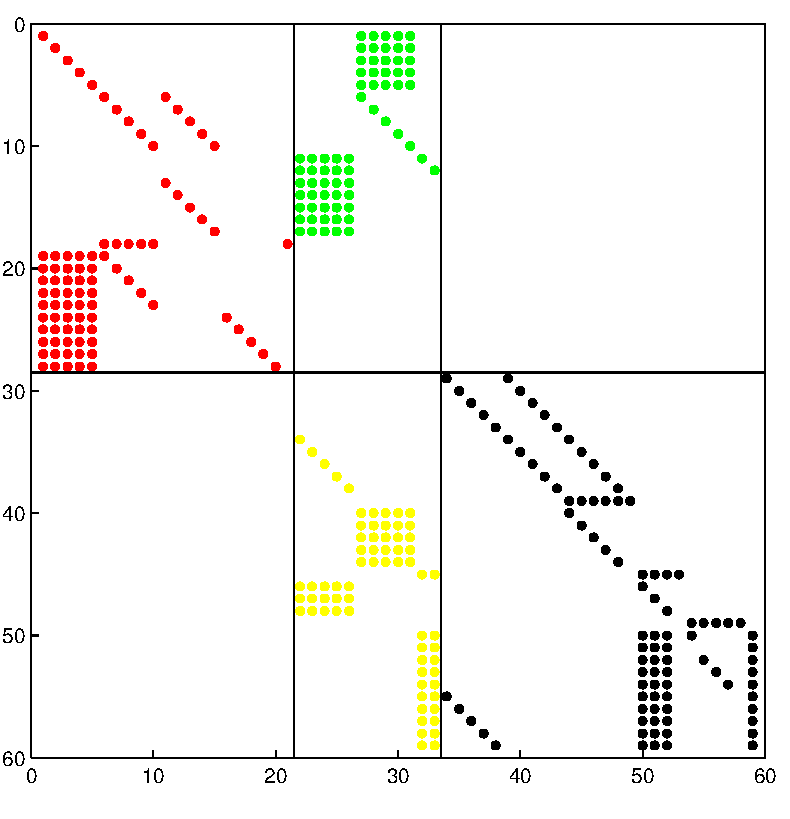
\includegraphics[scale=0.5]{img/impcol_b.pdf} \label{fig:impcol_b}} \hspace{1cm}
	\subfigure[\texttt{cage6}]{ 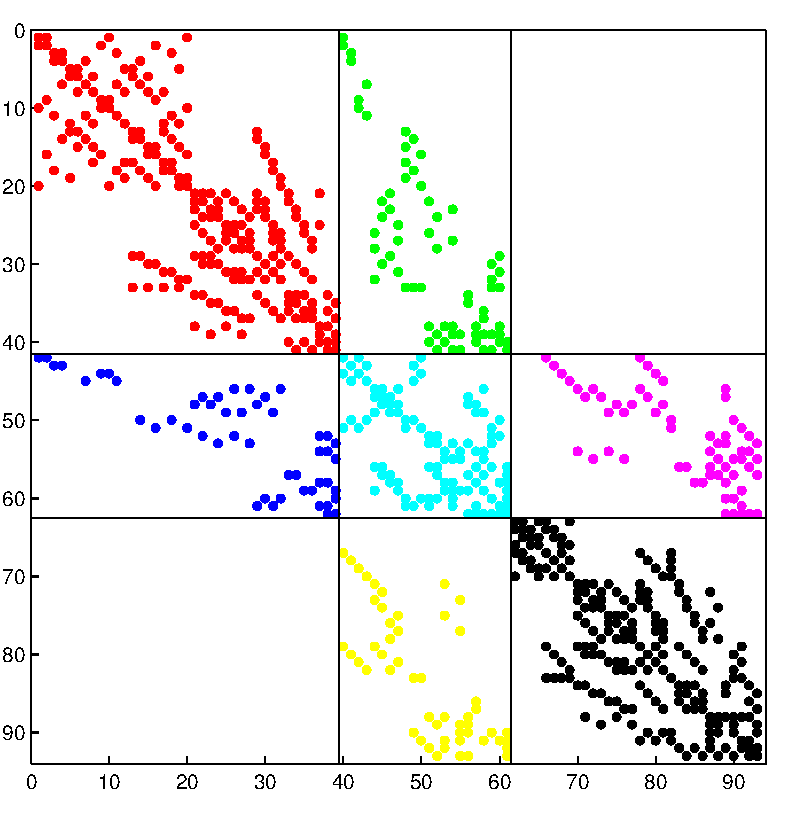
\includegraphics[scale=0.5]{img/cage6.pdf} \label{fig:cage6} }
	\caption{Example of SBD forms of partitioning of the matrices \texttt{impcol\_b} and \texttt{cage6} \cite{ufl}. Each part of $\dot{A}$ has been colored differently. In the first matrix there are no cut rows, which means that $\dot{A}_{10}=\dot{A}_{11} =\dot{A}_{12} = \varnothing$.} \label{fig:sbd-2}
\end{figure}

By computing the Separated Block Diagonal form of a matrix, we are able to explicitly see the underlying structure of the partitioning of a matrix, and the properties of each block can be used to adapt the assignment of its nonzeros. More specifically, the blocks $\dot{A}_{00}$ and $\dot{A}_{22}$ have nonzeros with uncut rows and columns and therefore are more suited to be assigned together; of course, we still have to decide between $A_r$ and $A_c$ and, as mentioned earlier, it is impossible to do both: it is convenient to base our choice on the sizes of such blocks. For example, if $m_0 < n_0$, in the block $\dot{A}_{00}$ the columns are (on average) sparser than the rows: if we assign the nonzeros of this block to $A_c$ we are, in principle, making sure that more rows/columns will stay uncut.

For the blocks with uncut rows and cut columns (namely, $\dot{A}_{01}$ and $\dot{A}_{21}$), the choice is easy: we assign them to $A_r$ and keep their rows uncut. Similarly, we assign the nonzeros of $\dot{A}_{10}$ and $\dot{A}_{12}$ to $A_c$, keeping their columns uncut. 

For the middle block $\dot{A}_{11}$, whose nonzeros have cut rows and cut columns, we cannot exploit any underlying structure: a possible way is to employ one of the other heuristics described in this chapter only considering this submatrix. Our choice is to go with Algorithm \ref{alg:localview-po} presented in Section \ref{sec:localview} (note that we cannot exploit the partition-aware variant of it, because all of the nonzeros in the block considered have cut rows and columns).

The heuristic that employs the SBD structure of a matrix can be explictly visualized in \eqref{eq:sbdview}.

\begin{align}
	\text{	Assignment of } \dot{A}:	\begin{bmatrix}
		R/C & R & \\
		C & M & C \\
		& R & R/C \\
	\end{bmatrix}
	\label{eq:sbdview}
\end{align}

In this matrix, whose structure is the same of \eqref{eq:sbd}, the letter $R$ in a block denotes that we assign that block to $A_r$, and similarly for $C$ and $A_c$. Moreover, $R/C$ stands that the choice between $A_r$ and $A_c$ depends on the block size, whereas $M$ indicates that the block is assigned in a mixed manner, according to Algorithm \ref{alg:localview-po}.

Note that, as mentioned in Chapter \ref{chap:introduction}, the matrix is usually split by means of recursive bipartitionings: it is then sufficient to keep track of the order of these recursions to have an implicit ordering which can be easily used to compute the SBD form of a matrix \cite{yzelman_cache}, instead of computing this form from scratch using the algorithm described in \cite[Appendix A]{bas}.

In Chapter \ref{chap:experimental_results}, we will refer to the algorithm described in this section as \verb|pa_sbdview|.

\subsection{Using the Separated Block Diagonal form of order 2 of $A$} \label{sec:sbd2}

The proposed SBD2 form of a partitioned matrix $A$ is an extension of the SBD form: given a partitioned matrix $A$, we compute the Separate Block Diagonal form of $A$ of order 2 by separating, in $\dot{A}_{10}$ and $\dot{A}_{12}$ the empty and non-empty columns, and in $\dot{A}_{01}$ and $\dot{A}_{21}$ the empty and non-empty rows. Then all the other blocks, except the central one, are permuted and split up accordingly. This procedure is better shown in Algorithm \ref{alg:sbd2}. 

\begin{algorithm}[h]
	\begin{algorithmic}
		\Require{ partitioned matrix $A$}
		\Ensure{$\ddot{A}$}
		\State compute $\dot{A}$ as the SBD form of $A$ and obtain also $R_0,R_1,R_2,C_0,C_1,C_2$;
		\State split $R_0$ in $R_{00}$ and $R_{01}$, such that $A(R_{00},C_1) = \varnothing$;
		\State split $R_2$ in $R_{20}$ and $R_{21}$, such that $A(R_{21},C_1) = \varnothing$;
		\State split $C_0$ in $C_{00}$ and $C_{01}$, such that $A(R_1,C_{00}) = \varnothing$;
		\State split $C_2$ in $C_{20}$ and $C_{21}$, such that $A(R_1,C_{21}) = \varnothing$;
		\State $I:= (R_{00},R_{01},R_1,R_{20},R_{21})$;
		\State $J:= (C_{00},C_{01},C_1,C_{20},C_{21})$;
		\State $\ddot{A} := A(I,J)$.
	\end{algorithmic}
	\caption{Algorithm to obtain SBD2 form of a matrix $A$.} \label{alg:sbd2}
\end{algorithm} 

The resulting final matrix is a block tridiagonal matrix $\ddot{A}$:

\begin{align}
	\ddot{A} := \begin{bmatrix}
		\ddot{A}_{00} & \ddot{A}_{01} & & & \\
		\ddot{A}_{10} & \ddot{A}_{11} & \ddot{A}_{12} & & \\
		& \ddot{A}_{21} & \ddot{A}_{22} & \ddot{A}_{23} & \\
		& & \ddot{A}_{32} & \ddot{A}_{33} & \ddot{A}_{34} \\
		& & & \ddot{A}_{43} & \ddot{A}_{44} \\
	\end{bmatrix},
	\label{eq:sbd2}
\end{align}

where each submatrix $\ddot{A}_{pq}$ is of size $m_p \times n_q$.

Figure \ref{fig:sbd2} shows the process of obtaining this matrix $\ddot{A}$ starting from the SBD matrix $\dot{A}$ obtained in Figure \ref{fig:sbd}.

\begin{figure}[h]
	\centering
	\begin{tikzpicture}[scale=0.5]
		\foreach \x / \y in {4/4,4/6,5/5,7/8,7/7,8/8,6/9,9/4} { \fill[myred] ({0+\y-1},{-\x+1}) rectangle +(1,-1);}
		\foreach \x / \y in {1/1,1/3,2/4,3/2,4/5,5/6,6/1} { \fill[myblue] ({0+\y-1},{-\x+1}) rectangle +(1,-1);}

%		\draw[help lines] (0,-9) grid ({0+9},0);
		\foreach \x / \y in {2/0,4/1,6/2,0/3,1/4,5/5,3/6,7/7,8/8} {\node at ({0+9.5},{-\y-.5}) {\x};}
		\foreach \x / \y in {5/0,7/1,8/2,0/3,1/4,2/5,3/6,4/7,6/8} {\node at ({0+\y+.5},-9.5) {\x};}

		\node at (1.5,-10.7) {$C_0$};
		\node at (4.5,-10.7) {$C_1$};
		\node at (7.5,-10.7) {$C_2$};

		\node at (11,-1.5) {$R_0$};
		\node at (11,-4.5) {$R_1$};
		\node at (11,-7.5) {$R_2$};

		\draw[very thick] ({0+0},-9) rectangle ({0+9},0);

		\draw[ultra thick] ({0+3},0) -- ({0+3},-9);
		\draw[ultra thick] ({0+6},0) -- ({0+6},-9);

		\draw[ultra thick] ({0+0},-3) -- ({0+9},-3);
		\draw[ultra thick] ({0+0},-6) -- ({0+9},-6);

		\draw[thick,myarrow] (13,-4.5) -- (17,-4.5);

		\foreach \x / \y in {4/4,4/6,5/5,8/9,8/8,9/9,6/7,7/4} { \fill[myred] ({19+\y-1},{-\x+1}) rectangle +(1,-1);}
		\foreach \x / \y in {1/3,1/2,3/4,2/1,4/5,5/6,6/3} { \fill[myblue] ({19+\y-1},{-\x+1}) rectangle +(1,-1);}

%		\draw[help lines] (19,-9) grid ({19+9},0);
		\foreach \x / \y in {2/0,6/1,4/2,0/3,1/4,5/5,8/6,3/7,7/8} {\node at ({19+9.5},{-\y-.5}) {\x};}
		\foreach \x / \y in {7/0,8/1,5/2,0/3,1/4,2/5,6/6,3/7,4/8} {\node at ({19+\y+.5},-9.5) {\x};}

		\node at ({19+1},-10.7) {$C_{00}$};
		\node at ({19+2.5},-10.7) {$C_{01}$};
		\node at ({19+4.5},-10.7) {$C_{1}$};
		\node at ({19+6.5},-10.7) {$C_{20}$};
		\node at ({19+8},-10.7) {$C_{21}$};

		\node at ({19+11},-1) {$R_{00}$};
		\node at ({19+11},-2.5) {$R_{01}$};
		\node at ({19+11},-4.5) {$R_{1}$};
		\node at ({19+11},-6.5) {$R_{20}$};
		\node at ({19+11},-8) {$R_{21}$};

		\draw[very thick] ({19+0},-9) rectangle ({19+9},0);

		\draw[ultra thick] ({19+3},0) -- ({19+3},-9);
		\draw[ultra thick] ({19+6},0) -- ({19+6},-9);
		\draw[ultra thick] ({19+2},0) -- ({19+2},-9);
		\draw[ultra thick] ({19+7},0) -- ({19+7},-9);

		\draw[ultra thick] ({19+0},-3) -- ({19+9},-3);
		\draw[ultra thick] ({19+0},-6) -- ({19+9},-6);
		\draw[ultra thick] ({19+0},-2) -- ({19+9},-2);
		\draw[ultra thick] ({19+0},-7) -- ({19+9},-7);
	\end{tikzpicture}
	\caption{SBD2 form obtained starting from the SBD form of Figure \ref{fig:sbd}.} \label{fig:sbd2}
\end{figure}

To better understand the interesting properties of the newly created parts of the matrix, let us introduce the concept of \emph{neighbor}: given the nonzero $a_{ij}$ we say that $a_{kl}$ is a neighbor if $k = i \vee l = j$; in other words, neighbors of a given nonzero are the ones that lie in the same row or in the same column.

Now, let us consider, for sake of brevity, just the top-left corner of $\ddot{A}$: nonzeros in $\ddot{A}_{00}$ are uncut in the rows and columns and whose neighbors are uncut also in the other, non-shared, dimension. Similarly, nonzeros in $\ddot{A}_{01}$ do not have any neighbor (w.r.t. their row) with cut columns but have neighbors (w.r.t their column) with cut rows. And similarly, with the roles of rows and columns reversed, for $\ddot{A}_{10}$. This exact same reasoning applies also for the bottom-right corner, with the appropriate adaptation of indices.

The size of these parts, and more generally of all of the blocks of $\ddot{A}$, is again highly dependent on the structure of the matrix, as shown in Figure \ref{fig:sbd2-2}.

\begin{figure}[h]
	\centering
	\subfigure[\texttt{impcol\_b}]{ 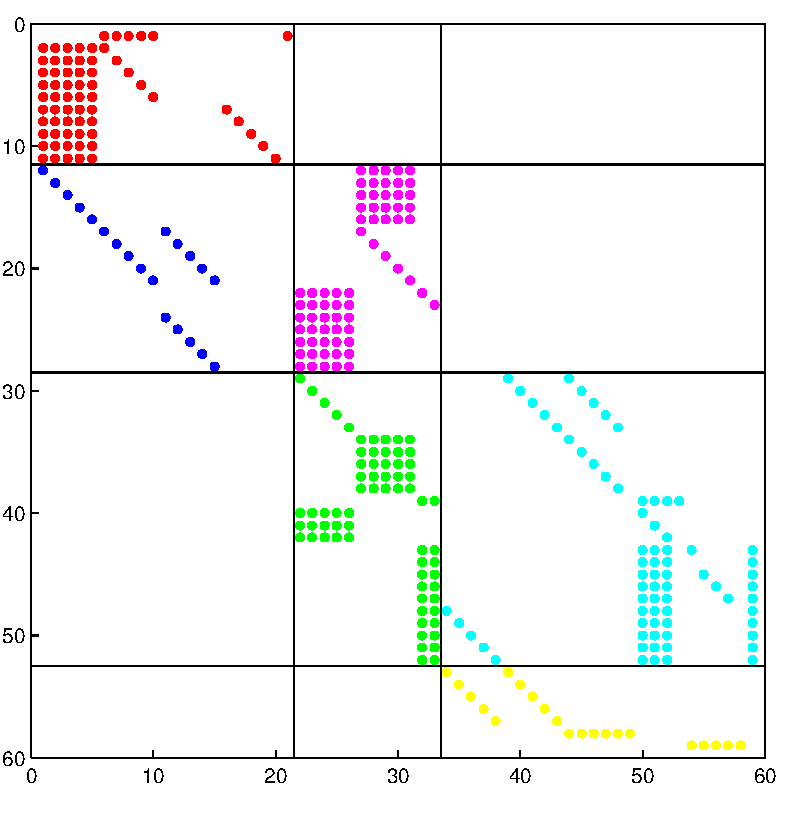
\includegraphics[scale=0.5]{img/sbd2_impcol_b.pdf} \label{fig:sbd2_impcol_b}}\hspace{1cm} 
	\subfigure[\texttt{cage6}]{ 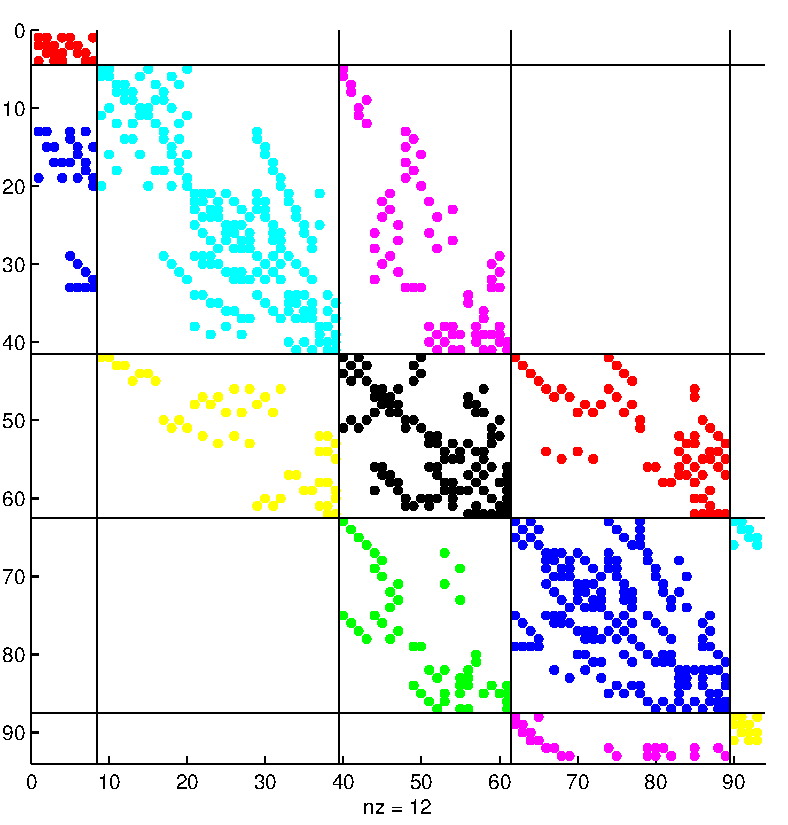
\includegraphics[scale=0.5]{img/sbd2_cage6.pdf} \label{fig:sbd2_cage6} }
	\subfigure[\texttt{sherman1}]{ 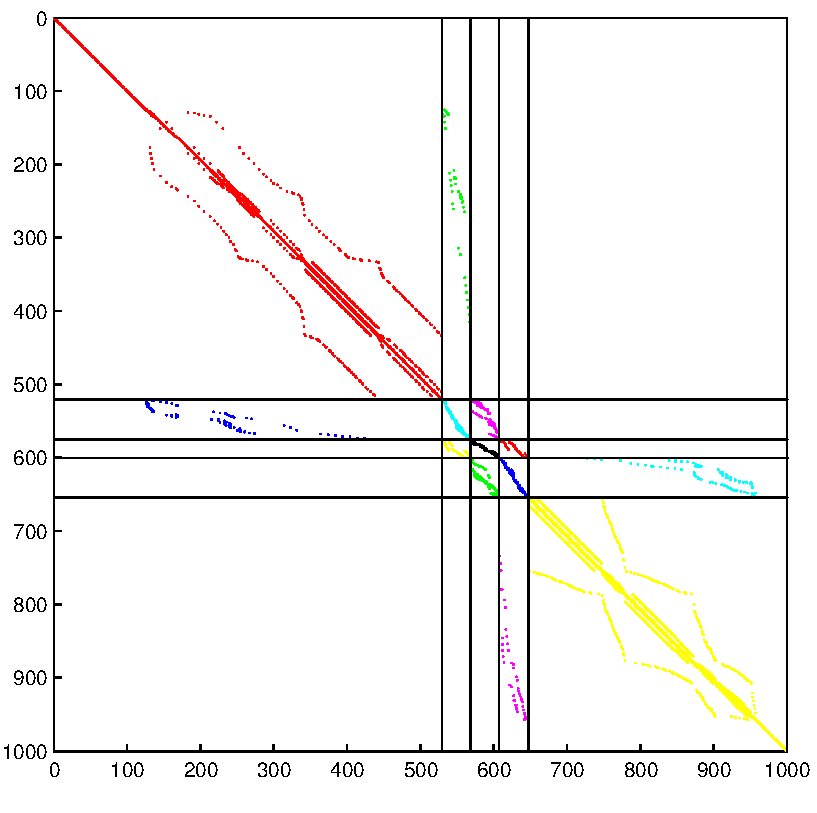
\includegraphics[scale=0.5]{img/sbd2_sherman1.pdf} \label{fig:sbd2_sherman1}} 
	\caption{Example of SBD2 forms of three different matrices. Similarly as in Figure \ref{fig:sbd-2}, each part of $\ddot{A}$ has been given a color (note that since there are more parts than coloris used, some colors are repeated even though the parts are not related in any way).	We can see in \ref{fig:sbd2_impcol_b} that the second and fourth columns are empty, and therefore not shown in the image. We can also see the difference in structure between \ref{fig:sbd2_cage6} and \ref{fig:sbd2_sherman1}: the former one comes from a DNA electrophoresis problem \cite{ufl}, while the latter is an oil reservoir simulation challenge matrix \cite{matrixmarket}. We can see that with the \texttt{sherman1} matrix, the corner parts are predominant because it is a finite element matrix, with a strongly diagonal pattern: it makes sense that most of these nonzeros are ``independent'' from each other. }  \label{fig:sbd2-2}
\end{figure}

Other than the corner blocks, for which we already argued that the matrix partitioning problem is easy, this structure enables us to assign more specifically nonzeros to either $A_r$ or $A_c$: it is convenient to assign $\ddot{A}_{01}$ and $\ddot{A}_{43}$ to $A_r$, as these nonzeros can be fully assigned to one processor without having the columns cut, and similarly we can assign $\ddot{A}_{10}$ and $\ddot{A}_{34}$ to $A_c$; for the other blocks, we can repeat the reasoning of the last section.

This heuristic that exploits the SBD2 form of the matrix $A$ is given explicitly as follows:

\begin{align}
	\text{Assignment of } \ddot{A}: \begin{bmatrix}
		R & R & & & \\
		C & R/C & R & & \\
		& C & M & C & \\
		& & R & R/C & C \\
		& & & R & C \\
	\end{bmatrix}
	\label{eq:sbd2view}
\end{align}

$R$ denotes, as previously, that the block as been assigned to $A_r$ and similarly for $C$ and $A_c$. $R/C$ denotes that the assignment depends on the block size and $M$ that a mixed assignment is performed with Algorithm \ref{alg:localview-po}.

Note that, in this case, the SBD2 form has to be computed from scratch from the SBD form, because it uses further information that is not employed during the normal partitioning.

In Chapter \ref{chap:experimental_results}, we will refer to the algorithm described in this section as \verb|pa_sbd2view|.

\section{Maximizing empty rows of $B$} \label{sec:globalview}

In this section, instead of describing a generating scheme that takes as input the matrix $A$ and produces as output $A_r$ and $A_c$, we will introduce an improvement scheme, which operates on already existing $A_r$ and $A_c$ and tries to refine them such that the upper bound on the communication volume is lowered.

At the beginning of this chapter, we mentioned how it is convenient to have full rows assigned to $A_r$ and full columns assigned to $A_c$, in order to avoid communication; a good strategy to produce good $A_r$ and $A_c$, could then be to maximize such full assignments. The proposed heuristic does essentially this, by trying to swap the assignment of nonzeros from $A_r$ to $A_c$ and viceversa, trying to obtain that full rows are assigned to $A_r$ and full columns are assigned to $A_c$. In order to achieve both of these goals with a unique algorithm, it is convenient to reason in terms of the matrix $B$ as in \eqref{eq:Bmatrix}. If we maximize the number of empty rows of $B$, we are effectively emptying rows of $A_r^T$ (i.e. emptying columns of $A_r$, therefore fully assigning nonzeros in them to $A_c$) and of $A_c$, thus assigning full rows to $A_r$.

This improvement heuristic falls into the category of \emph{local search} algorithms: we start from a configuration (an assignment of nonzeros to $A_r$ and $A_c$) and perform a search on the neighborhood, defined as the set of configurations which differ only by the assignment of a single nonzero. By performing this small swap, we can easily fall in a local optimum situation: a few nonzeros (depending on the structure of the matrix) are continuously swapped between $A_r$ and $A_c$. 

We can add a little hill-climbing capability to our heuristic by adding a little buffer: we pre-determine $l_{max}$, the maximum amount of worsening allowed, and, after this threshold is reached, we start considering only strictly improving solution. In order to have a meaningful threshold, it might be convenient to have it relative to the amount of rows/columns of $B$, or to its nonzeros. The higher this threshold is, the more capability we have of escaping local optima, but at the cost of slowing down considerably the improvement (even potentially arresting it) of our solution.

For the choice of the neighbor configuration to consider, it is convenient to consider the row of $B$ with a diagonal element (which corresponds to a split row/column of $A$) with the minimum number of nonzeros: our immediate goal, which in reality spans over a few moves of our local search, is to fully assign the nonzeros of this row of $B$; we consider the minimum because each time we swap we might slightly worsen the solution.

A more explicit overview on this local search improvement scheme is described in Algorithm \ref{alg:globalview}:

\begin{algorithm}[h]
	\begin{algorithmic}
		\Require{$A_r$, $A_c$, $l_{max}$, $iter_{max}$}
		\Ensure{$A_r'$, $A_c'$}
		\State $l := 0$
		\State Compute $B$ following the medium-grain model
		\For{$it=1,\dots,iter_{max}$}
		\State $\displaystyle i := \argmin_{k \in \{1,\dots,m+n\}\text{ s.t. }B(k,k) \neq 0} nz_r(k)$
		\ForAll{$j \neq i$ such that $B(i,j) \neq 0$}
		\If{$B(j,j) \neq 0$} 
		\State $B(i,j) = 0$
		\State $B(j,i) = 1$
		\Else
		\If{$l < l_{max}$}
		\State $B(i,j) = 0$
		\State $B(j,i) = 1$
		\State $l = l+1$
		\EndIf
		\EndIf
		\EndFor
		\If{$nz(B(i)) = 1$}
		\State $B(i,i) = 0$
		\State $l = l-1$
		\EndIf
		\EndFor
		\State $A_r' := B([1,\dots,n],[n+1,\dots,m+n])^T$
		\State $A_c' := B([n+1,\dots,m+n],[1,\dots,n])$	
	\end{algorithmic}
	\caption{Local search refinement of $A_r$ and $A_c$} \label{alg:globalview}
\end{algorithm}

As this is a scheme that relies on existing $A_r$ and $A_c$ and aims at improving them, we still need to choose how to generate these parts in the first place. If we can rely on an existing partitioning, a simple choice could be to take as $A_r$ and $A_c$ the subsets of nonzeros assigned, respectively, to processor 0 and 1; otherwise, if our goal is to produce $A_r$ and $A_c$ for the initial partitioning, the simplest choice is to randomly assign each nonzero to either $A_r$ or $A_c$. These initial solutions, however, are fast to generate but not particularly efficient, and are therefore meaningful only if our improvement scheme is fast enough; otherwise, we can always rely on one of the other heuristics described in this chapter.

\section{Partial assignment of rows and columns} \label{sec:hot_restart}

In Section \ref{sec:localview} we discussed how to assign each nonzero independently, whereas in Section \ref{sec:sbd} we examined the possibility of exploiting a little the structure of the matrix, in order to assign more nonzeros at once. Keeping this direction, there is some other structure of $A$ that can lead to a better assignment: partial assignment of rows and columns.

The main idea behind this heuristic is that, every time we assign a nonzero to $A_r$, we know that it is convenient that also all the other nonzeros in the same row are assigned to it; conversely, if a nonzero is assigned to $A_c$, all the nonzeros in its column should stick with it. Therefore, we ideally want to keep together rows and columns as much as possible; but, as already discussed, there is always the problem that a nonzero cannot be assigned to both $A_r$ and $A_c$, we can only reason in term of partial assigment of the row/column. 

Throughout this section we will stop distinguishing between rows and columns of a matrix and reason in term of \textbf{indices} in the set $\{0,\dots,m+n-1\}$: following the natural ordering, the $m$ rows are mapped to $0,\dots,m-1$ and the $n$ columns to $m,\dots,m+n-1$.

This simplification of terms is due to the fact that the core of this heuristic lies in the computation of a \textbf{priority vector} $v$, which is none other than a permutation of the indices $0,\dots,m+n-1$, where they appear in order of decreasing priority: in this sense, the priority is to be intended as the probability of the nonzeros of that index to be together in a good partitioning.

The assignment of nonzeros is done by ``painting'' them with an imaginary color, which corresponds either to $A_r$ or $A_c$: we iterate through our priority vector backwards (i.e. starting from the index with the lowest priority) and assign all of its nonzeros to go together: if the index corresponds to a row, then we assign all of its nonzeros to $A_r$, otherwise we assign them to $A_c$. Because each nonzero has both a row and a column, it is represented twice in our priority vector; the second time it is considered, we re-assign it by ``painting it over'' (hence the name of the algorithm).

A more explicit formulation of this procedure is given in Algorithm \ref{alg:overpainting}.

\begin{algorithm}[h]
	\begin{algorithmic}
		\Require{Priority vector $v$, matrix $A$}
		\Ensure{$A_r$, $A_c$}
		\State $A_r := A_c: = \varnothing$
		\For{$i=m+n-1,\dots,0$}
		\If{$v_i < m$}
		\State Add the nonzeros of row $i$ to $A_r$
		\Else
		\State Add the nonzeros of column $i$ to $A_c$
		\EndIf
		\EndFor
	\end{algorithmic}
	\caption{Overpainting algorithm} \label{alg:overpainting}
\end{algorithm}

It is possible also to give an alternative formulation for this algorithm in which we iterate forward through $v$, as described in Algorithm \ref{alg:overpainting-2}.

\begin{algorithm}[h]
	\begin{algorithmic}
		\Require{Priority vector $v$, matrix $A$}
		\Ensure{$A_r$, $A_c$}
		\State $A_r := A_c: = \varnothing$
		\For{$i=0,\dots,m+n-1$}
		\If{$v_i < m$}
		\State Add the unmarked nonzeros of the row $i$ of $A$ to $A_r$
		\Else
		\State Add the unmarked nonzeros of the column $i$ of $A$ to $A_c$
		\EndIf
		\State Mark nonzeros of index $i$ as ``evaluated''
		\EndFor
	\end{algorithmic}
	\caption{Alternative formulation of Algorithm \ref{alg:overpainting}.} \label{alg:overpainting-2}
\end{algorithm}

In this formulation, every assignment to $A_r$ and $A_c$ is final, but with the added complexity of checking which nonzeros of the considered index are still to be assigned, and only work with them.

Lastly, another different formulation is possible: we consider individually each nonzero $a_{ij}$ and see whether in $v$ $i < j$ (where the $<$ symbol is to be intended as ``$i$ precedes $j$'' and not as the comparison of the values) or the other way around; in the first case, the row has more priority and we assign $a_{ij}$ to $A_r$, otherwise we assign it to $A_c$. Note that, since we have to perform $N$ lookups on the vector $v$, this is a more expensive formulation of the same algorithm.

An important point to observe is that this overpainting algorithm is completely deterministic: $A_r$ and $A_c$ are uniquely determined by the ordering of the indices in $v$. Therefore, the heuristic part of this algorithm lies entirely in the choice of this priority vector, and, for this reason, we will focus on it in the next subsection. 

\subsection{Computation of the priority vector $v$}

Because, with the overpainting algorithm, the quality of $A_r$ and $A_c$ depends entirely on the choice of $v$, it is important to take a structured approach and explore a wide variety of possibilities for this priority vector.

In this section, we proceed and define several \emph{generating schemes}, and their input determines whether the overpainting algorithm is used to obtain a better initial partitioning or a fully iterative scheme. In general, we try to come up with schemes that can be used for either purpose, with slight modifications. 

Each one of the generating schemes can be summarized in three main steps:

\begin{enumerate}
	\item usage of previous partitioning;
	\item sorting;
	\item internal ordering of indices.
\end{enumerate}

Now, we give a more detailed explanation of each of those steps. 

\begin{itemize}
	\item \textbf{usage of previous partitioning}: if we are considering \emph{partition aware generating schemes}, we separate the set of uncut indices (i.e. indices which correspond to uncut rows or columns) from the  cut indices. We consider the simple concatenation of uncut indices and cut indices, in this order, and the next steps are performed on each of these parts. If, instead, we are considering a \emph{partition oblivious scheme}, the subsequent operations are performed on the set $\{0,\dots,m+n-1\}$.

	\item \textbf{sorting}: we can either keep the set from the previous step untouched (therefore preserving the natural order of indices) or perform a sorting with respect to the number of nonzeros. The sorting is done in ascending order, as a short row/column is more likely to fit completely in a good partitioning because it does not yield many cut columns/rows.

		In addition, we can refine a bit our sorting: we could move the indices which have only one nonzero to the back, because no matter our assignment of such nonzero, that index will not be cut and it is best to try to keep also the other dimension uncut. 

	\item \textbf{internal ordering}: as the last step, we want to finalize our vector $v$ by deciding more precisely the position of each index. The strategies considered, which often depend internally on an additional parameter, are the following:

		\begin{itemize}
			\item \textbf{concatenation}: we put either all the rows before all the columns, or all the columns before all the rows;
			\item \textbf{mixing}: we can mix rows and columns in two main ways: alternation and spread. Suppose there are twice as many columns as rows: in the first case we get
				$$(c,r,c,r,c,r,\dots,c,r,c,c,c,\dots,c,c,c),$$

				whereas with the second one we get 

				$$(c,c,r,c,c,r,\dots,c,c,r),$$

				where with $c$ we denote a generic column and with $r$ a generic row. To obtain a more even distribution, we always start with the greater dimension.
			\item \textbf{random} (only in case of no sorting): we randomize the ordering of the indices;
			\item \textbf{simple} (only in case of sorting): we let the sorting decide completely the ordering, and the vector is left as is.
		\end{itemize}
\end{itemize}

As the complete description of a generating scheme is somewhat lengthy, we use a simplified notation and adopt the following abbreviations:

\begin{itemize}
	\item \verb|PO|: partition oblivious
	\item \verb|PA|: partition aware
	\item \verb|sorted| and \verb|unsorted|: sorting w.r.t. the number of nonzeros is performed or not
	\item \verb|w| and \verb|nw|: all the indices with only 1 nonzero are moved to the back or not
	\item \verb|simple|: the sorted vector is left as-is
	\item \verb|concat|: rows and columns are concatenated
	\item \verb|row|: the concatenation is done rows-columns
	\item \verb|col|: the concatenation is done columns-rows
	\item \verb|mix|: mixing of the rows and columns is enforced
	\item \verb|alt|: rows and columns are alternated
	\item \verb|spr|: rows and columns are spread
	\item \verb|random|: the order of the indices is randomized
\end{itemize}

With this notation, the name \verb|po_sorted_nw_mix_spr| stands for ``partition oblivious generating scheme, with indices sorted by number of nonzeros, without moving the indices with 1 nonzero to the back, with forced mixing of rows and columns, in a spread fashion''. This is just one of the many possibilities, which are convenient to visualize using a directed graph, as shown in Figure \ref{fig:digraph}; a generating scheme is simply a path from START to END. 

\begin{figure}[h]
	\begin{center}
		\begin{tikzpicture}[every path/.style={>=latex}]
			\node (start) at (6,14) {START};
			\node (po) at (4.5,12.5)  { PO };
			\node (pa) at (7.5,12.5) { PA };
			\node (d1) at (6,11.5) {$\bullet$};
			\node (sorted) at (3,9.5) {sorted};
			\node (unsorted) at (10.5,9.5) {unsorted};
			\node (w) at (2,8.25) {w};
			\node (nw) at (4,8.25) {nw};
			\node (d3pre) at (3,7) {$\bullet$};
			\node (d3) at (6,5) {$\bullet$};
			\node (concat) at (4.5,3) {concat}; 
			\node (mix) at (7,3) {mix};
			\node (random) at (10.5,3) {random};
			\node (simple) at (1,3) {simple};
			\node (alt) at (6.5,2) {alt};
			\node (row) at (4,2) {row};
			\node (col) at (5,2) {col};
			\node (end) at (6,-0.5) {END};
			\node (spr) at (7.5,2) {spr};

			\draw[->] (start) edge (po);
			\draw[->] (start) edge (pa);

			\draw[->] (po) edge (d1);
			\draw[->] (pa) edge (d1);

			\draw[->] (d1) edge (sorted);
			\draw[->] (d1) edge (unsorted);

			\draw[->] (sorted) edge (w);
			\draw[->] (sorted) edge (nw);

			\draw[->] (unsorted) edge (d3);
			\draw[->] (w) edge (d3pre);
			\draw[->] (nw) edge (d3pre);
			\draw[->] (d3pre) edge (d3);
			\draw[->] (d3pre) edge (simple);

			\draw[->] (d3) edge (mix);
			\draw[->] (d3) edge (concat);

			\draw[->] (unsorted) edge (random);

			\draw[->] (mix) edge (alt);
			\draw[->] (mix) edge (spr);

			\draw[->] (alt) edge (end);
			\draw[->] (spr) edge (end);

			\draw[->] (concat) edge (row);
			\draw[->] (concat) edge (col);

			\draw[->] (row) edge (end);
			\draw[->] (col) edge (end);
			\draw[->] (simple) edge (end);
			\draw[->] (random) edge (end);

			\draw[dashed] (0,13.25) -- (13,13.25);
			\draw[dashed] (0,10.5) -- (13,10.5);
			\draw[dashed] (0,4) -- (13,4);
			\draw[dashed] (0,0.5) -- (13,0.5);

			\node[align=left,draw] at (13,12) {usage of previous \\partitioning};
			\node[align=left,draw] at (13,7) {sorting};
			\node[align=left,draw] at (13,2) {internal ordering};
		\end{tikzpicture}
	\end{center}
	\caption{Directed graph that represents the family of heuristics used (any path from START to END). Dummy nodes (the ones without any label) were added in order to reduce the number of edges and ease legibility.} \label{fig:digraph}
\end{figure}

Other than this family of heuristics, we can also formulate the problem of partial assignment of rows/columns, always following this framework, in another more mathematical way, to which we dedicate Chapter \ref{chap:independent_set}.
